\documentclass[12pt,twoside,book]{article}
\usepackage{docmute}

\input{../settings}

\begin{document}

%%%%%%%%%%%%%%%%%%%%%%%%%%%%%%%%%%%%%%%%%%%%%%%%%%%%%%%%%%%%%%%%%%%%%%%%%%%%%%%
\section{Direct collider search of WIMPs}
\setcounter{equation}{0}
%%%%%%%%%%%%%%%%%%%%%%%%%%%%%%%%%%%%%%%%%%%%%%%%%%%%%%%%%%%%%%%%%%%%%%%%%%%%%%%

\vskip 0.1in

In this section, we review the production of $\mathrm{TeV}$-scale WIMPs and search for their signals using the collider experiment.
In particular, we will summarize the current bounds for WIMPs obtained at the large hadron collider (LHC) and future bounds expected at the future planned $100\,\mathrm{TeV}$ colliders such as the hadron option of the future circular collider (FCC-hh) \cite{Benedikt:2651300} and the super proton-proton collider (SPPC) \cite{CEPC-SPPCStudyGroup:2015csa, CEPC-SPPCStudyGroup:2015esa}.
In Sec.~\ref{sec:wimp_production}, we discuss the dominant production processes of WIMPs at a hadron collider.
In Sec.~\ref{sec:disappearing_track} and \rem{???}, we review \rem{two???} different methods for the signal identification, the disappearing track search and mono-jet search \rem{???}, and summarize the current and future bounds.


%%%%%%%%%%%%%%%%%%%%%%%%%%%%%%%%%%%%%%%%%%%%%%%%%%%%%%%%%%%%%%%%%%%%%%%%%%%%%%%
\subsection{WIMP production}
\label{sec:wimp_production}
%%%%%%%%%%%%%%%%%%%%%%%%%%%%%%%%%%%%%%%%%%%%%%%%%%%%%%%%%%%%%%%%%%%%%%%%%%%%%%%

There are two relevant processes both of which significantly contribute to the WIMP production cross section.
The pair production via electroweak interaction is a universal process that can be considered for any WIMP considered in this thesis.
The decay of colored particles may also be efficient particularly for the MSSM.
In this subsection, we will review these two in order.


\subsubsection*{Pair production via electroweak interaction}

\begin{figure}[b]
  \centering
  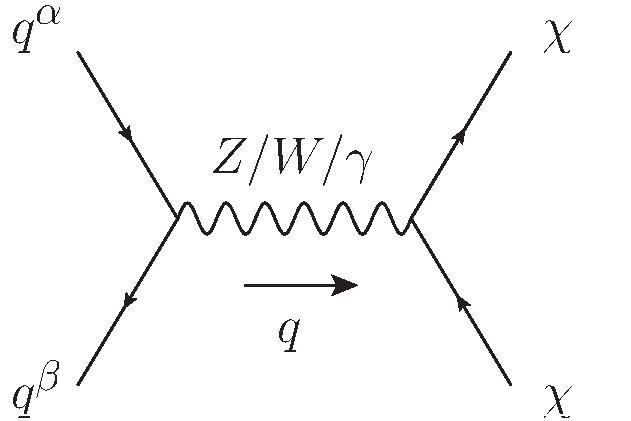
\includegraphics[width=0.4\hsize]{WIMP_production.pdf}
  \caption{WIMP pair production process at the hadron collider.}
  \label{fig:wimp_production}
\end{figure}

Since all the WIMPs considered here possess non-zero $SU(2)_L$ and $U(1)_Y$ charges, they can be directly produced via electroweak interaction at the hadron collider as shown in Fig.~\ref{fig:wimp_production}.
\footnote{
  All the Feynman diagrams in this thesis are drawn with the public code \texttt{JaxoDraw-2.1} \cite{BINOSI20091709}, which is a graphical user interface that allows users to draw Feynman diagrams intuitively and export them in the \texttt{eps} format with the help of the (modification of) \texttt{axodraw} style file for \LaTeX \cite{VERMASEREN199445}.
  Under the environment of macOS Mojave, it apparently fails to start, but one can still execute it by looking inside the application and start the Java executable file \texttt{jaxodraw-2.1-0.jar} directly.
  The author of this thesis would like to thank the authors for providing the best tools to write the thesis with.
  \rem{Correct here?}
}
In the figure, $q^\alpha$ and $q^\beta$ denote the partons (namely, one of quarks or gluon) of the incident protons relevant for the process, while $\chi$ denotes the WIMP and $q$ is the momentum transfer.
Assuming the WIMP to be a $SU(2)_L$ $n$-plet with $U(1)_Y$ charge $Y$ and the mass $m_\chi$, this process is well described by the effective lagrangian
\footnote{
  In this subsection, we neglect the small mass difference among different components in the multiplet $\chi$ described in \ref{sec:disappearing_track}.
  This approximation is valid since the mass difference is by far smaller than $m_\chi$ and has only a tiny effect on the production process.
}
\begin{align}
  \mathcal{L} &= \mathcal{L}_{\mathrm{SM}} + (D^\mu \chi)^\dagger (D_\mu \chi) - m_\chi^2 \chi^\dagger \chi &
  &\text{(complex scalar)}, \label{eq:lag_scalar}\\
  \mathcal{L} &= \mathcal{L}_{\mathrm{SM}} + \bar{\chi} (i \Slash{D} - m_\chi) \chi &
  &\text{(Dirac fermion)}, \label{eq:lag_fermion}
\end{align}
with $\mathcal{L}_{\mathrm{SM}}$ being the SM lagrangian, while the covariant derivative is given by
\begin{align}
  D_\mu \equiv \partial_\mu - i g_2 \Slash{W}^a T_n^a - i g_1 Y \Slash{B},
\end{align}
where $T_n^a$ ($a=1,2,3$) are $n$-dimensional representation matrices of $SU(2)_L$.
Note that when $\chi$ is a real scalar (Majorana fermion) with $Y=0$, the terms with $\chi$ in Eq.~\eqref{eq:lag_scalar} (Eq.~\eqref{eq:lag_fermion}) should be devided by two.

For the calculation, we neglect the effect of the electroweak symmetry breaking, which is valid because we are interested in the high-energy collision with the parton-level center-of-mass (CM) energy $\sqrt{s'} \equiv \sqrt{q^2} \gsim \mathrm{TeV}$.
Then, we consider the process in the CM frame and estimate the parton-level differential cross section as
\begin{align}
  \left. \frac{d \sigma_{\alpha \beta}}{d \sqrt{s'} d \Omega} \right|_{\text{CM}}
  &= \frac{C_{\alpha \beta}}{8 s'} \left( 1 - \frac{4 m_\chi^2}{s'} \right)^{3/2} \sin^2 \theta
  & &(\text{complex scalar})\\
  \left. \frac{d \sigma_{\alpha \beta}}{d \sqrt{s'} d \Omega} \right|_{\text{CM}}
  &= \frac{C_{\alpha \beta}}{4 s'} \sqrt{1 - \frac{4 m_\chi^2}{s'}}
  \left[ 1 + \frac{4 m_\chi^2}{s'} + \left( 1 - \frac{4 m_\chi^2}{s'} \right) \cos^2 \theta \right]
  & &(\text{Dirac fermion}),
\end{align}
where $\theta$ is the angle between the momentum of the initial parton $q_a$ and that of one of the final state WIMPs.
Note that this expression represents an inclusive cross section, \textit{i.e.} the total cross section for the production of any component of the WIMP multiplet $\chi$.
The coefficient $C_{\alpha \beta}$ consists of contributions from $U(1)_Y$ and $SU(2)_L$ gauge bosons,
\footnote{
  There is no contribution from the interference term between $U(1)_Y$ and $SU(2)_L$ contributions, since it is proportional to $\mathrm{Tr} (T^a_n) = 0$.
}
\begin{align}
  C_{\alpha \beta} = c_{1 \alpha \beta} Y^2 \alpha_1^2
  + c_{2 \alpha \beta} I(n) \alpha_2^2,
\end{align}
with $I(n)$ being the Dynkin index for the $n$-dimensional representation given by
\begin{align}
  I(n) \equiv \frac{n^3-n}{12}.
  \label{eq:dynkin}
\end{align}
The explicit form of $c_{1 \alpha \beta}$ and $c_{2 \alpha \beta}$, which are sizes of the couplings between partons of our choice and gauge bosons, can be expressed using the $U(1)_Y$ charge for a parton $Y_\alpha$ and the $SU(2)_L$ reducible 13-dimensional representation matrices for partons $T^a_{\alpha \beta}$ as
\begin{align}
  c_{1 \alpha \beta} &= Y_\alpha^2 \delta_{\alpha \beta},\\
  c_{2 \alpha \beta} &= \sum_a \left| T^a_{\alpha \beta} \right|^2.
\end{align}
Recalling that $\alpha_1 < \alpha_2$ and that we often consider the WIMPs with large $n$ and moderate $Y$, the WIMP production cross section grows as $n^3$ for larger multiplets according to Eq.~\eqref{eq:dynkin}.

As is well-known, the initial state of the hadron collider is not the individual partons but two protons.
To obtain the cross section for the two protons initial state, we rely on the parton distribution function (PDF), which expresses the fraction of the partons with some given momentum in each accelerated proton.
Let $f_a (x)$ ($0 < x < 1$) be the PDF for a given parton $a$ inside a proton with momentum $p^\mu$.
$f_a (x)$ can be interpreted as a probability distribution to find the parton $a$ with momentum $x p^\mu$, so we have a relationship
\begin{align}
  \sum_a \int_0^1 dx \, x f_a (x) = 1,
\end{align}
associated with the total momentum conservation, and
\begin{align}
  \int_0^1 dx \, \left[ f_d (x) - f_{\bar{d}} (x) \right] &= 1,\\
  \int_0^1 dx \, \left[ f_u (x) - f_{\bar{u}} (x) \right] &= 2,
\end{align}
from the composition of the proton.
Using the PDF, the cross section for the process of interest at the hadron collider is evaluated as
\begin{align}
  \frac{d \sigma}{d \sqrt{s'} d \Omega} =
  \sum_{a,b} \int_0^1 dx_1 dx_2 \, f_a (x_1) f_b (x_2) \delta \left( s' - s x_1 x_2 \right)
  \left. \frac{d \sigma_{a b}}{d \Omega} \right|_{\text{lab}},
\end{align}
where $\sqrt{s}$ is the CM energy of the proton-proton collision.
Note that the cross section in the integrand is a function of $x_1$ and $x_2$, which is obtained by performing the appropriate Lorentz transformation to $\left. d \sigma_{a b} / d \Omega\, \right|_{\text{CM}}$.
\rem{Comment on factorization scale?}

\begin{figure}[t]
  \centering
  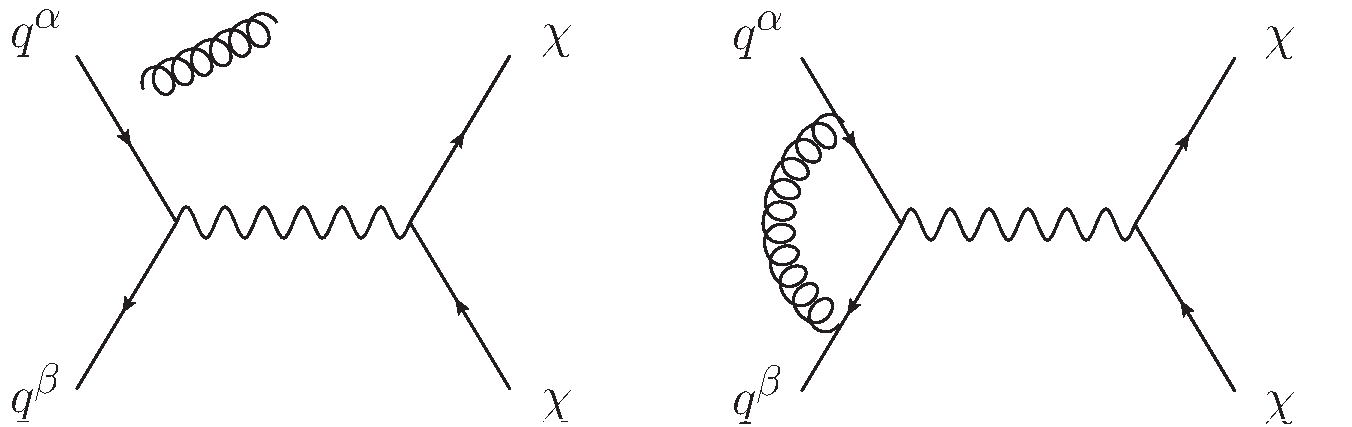
\includegraphics[width=0.8\hsize]{WIMP_production_NLO.pdf}
  \caption{Example of NLO QCD contributions to the WIMP pair production process.}
  \label{fig:WIMP_production_NLO}
\end{figure}

Hadron colliders have several more features related to the strong interaction of quantum chromodynamics (QCD).
Firstly, the next-to-leading order (NLO) QCD contribution to each process is not necessarily negligible.
For the WIMP pair production, the real and virtual emission of a gluon shown in the left and right panels of Fig.~\ref{fig:WIMP_production_NLO}, respectively, give the NLO QCD contributions, which will also be taken into account from now on.
In particular, when the large transverse momentum is important for the phenomenology of our concern, such as the case in Sec.~\rem{???}, the real emission of a gluon with sizable transverse momentum significantly modifies the calculation.
Secondly, all the colored particles in the initial, intermediate, and final states should be accompanied with numbers of soft emissions of gluons, which is the phenomena so-called the parton shower.
In practice, there is a difficulty caused by the partial overlap of the gluon phase space between the one-gluon emission cross section considered as an NLO QCD effect and the same considered as the parton shower.
To avoid this overlap, we often perform the matching procedure, in which we set some merging energy scale by hand and include the contribution to the cross section with gluon energy above (below) the scale only from the NLO QCD (parton shower) calculation.
Finally, the colored particles in the final states should eventually be confined, which is called the hadronization, and observed as some energetic and collimated sprays of hadrons, which as a whole is called jets.

In the following, we perform the numerical calculation, taking account of all the above complexities.
For this purpose, we make use of the Monte Carlo generator \texttt{MadGraph5 aMC@NLO (v2.6.3.2)} \cite{Alwall:2011uj,Alwall:2014hca} with the successive use of \texttt{Pythia8} \cite{Sjostrand:2014zea} for the parton shower, hadronization, and matching and \texttt{Delphes (v3.4.1)} \cite{deFavereau:2013fsa} for the detector simulation, including the definition of jets as observed objects.
We use the so-called MLM-style matching \cite{Mangano:2006rw} with the merging scale of $67.5\,\mathrm{GeV}$ and \texttt{NNPDF2.3QED} with $\alpha_3 (M_Z) = 0.118$ \cite{Ball:2013hta} as a canonical set of PDFs.
% For the renormalization and factorization scales, we adopt the default values of MadGraph5 aMC@NLO, \textit{i.e.}, the central $m^2_T$ scale after $k_T$-clustering of the event.

\begin{table}[t]
  \centering
  \begin{tabular}{c|cccc}
    WIMP name & Higgsino & Wino & $5$-plet Majorana fermion & $5$-plet real scalar \\ \hline
    $\sigma_{\mathrm{LO}}$ $[\mathrm{pb}]$ & 0.015 & 0.052 & \rem{???} & \rem{???} \\
    $\sigma_{\mathrm{NLO}}$ $[\mathrm{pb}]$ & 0.018 & 0.060 & \rem{???} & \rem{???} \\ \hline
    $K$-factor & 1.17 & 1.15 & &
  \end{tabular}
  \caption{
    Table of pair production cross sections of several types of WIMPs.
    The CM energy $\sqrt{s} = 100\,\mathrm{TeV}$ is assumed and WIMP masses are set to be $1\,\mathrm{TeV}$.
  }
  \label{tab:cross_section_WIMPs}
\end{table}

In Table~\ref{tab:cross_section_WIMPs}, we list the production cross sections of various WIMPs via a weak gauge boson exchange at a $\sqrt{s} = 100\,\mathrm{TeV}$ hadron collider.
As for the WIMP mass, we use the common value $m = 1\,\mathrm{TeV}$ to compare the cross sections among different choice of quantum numbers.
$\sigma_{\mathrm{LO}}$ and $\sigma_{\mathrm{NLO}}$ denote the production cross sections without and with the NLO QCD correction, respectively, while the last line is the so-called $K$-factor defined as $K = \sigma_{\mathrm{NLO}} / \sigma_{\mathrm{LO}}$.
From the table, by paying attention to the factor two difference in degrees of freedom between the Dirac (Higgsino) and Majorana (Wino and $5$-plet) fermions, we can roughly see the dependence of the cross section on the $SU(2)_L$ charge $\sigma \propto n^3$.
\rem{Correct? Seems that Higgsino cross section is too small?}

\begin{table}[t]
  \centering
  \begin{tabular}{c|cccc}
    Wino mass $\mathrm{[TeV]}$ & 1.0 & 1.5 & 2.0 & 2.9 \\ \hline
    $\sigma_{\mathrm{LO}}$ $[\mathrm{pb}]$ & 0.052 & 0.012 & 0.0040 & 0.00086\\
    $\sigma_{\mathrm{NLO}}$ $[\mathrm{pb}]$ & 0.060 & 0.015 & 0.0047 & 0.0010 \\ \hline
    $K$-factor & 1.15 & 1.20 & 1.19 & 1.21
  \end{tabular}
  \caption{
    Table of pair production cross sections of Wino with several choice of masses.
    The CM energy $\sqrt{s} = 100\,\mathrm{TeV}$ is assumed.
  }
  \label{tab:cross_section_Wino_mass}
\end{table}

\rem{Histogram of angular dependence}

\rem{Is angular dependence affected by the Lorentz boost?}

\subsubsection*{Decay of colored particles}


%%%%%%%%%%%%%%%%%%%%%%%%%%%%%%%%%%%%%%%%%%%%%%%%%%%%%%%%%%%%%%%%%%%%%%%%%%%%%%%
\subsection{Disappearing track search}
\label{sec:disappearing_track}
%%%%%%%%%%%%%%%%%%%%%%%%%%%%%%%%%%%%%%%%%%%%%%%%%%%%%%%%%%%%%%%%%%%%%%%%%%%%%%%

\rem{Histogram of surviving probability}

\rem{Histogram of beta distribution before / after 10cm cut}

\bibliographystyle{elsarticle-num}
\bibliography{../phd}

\end{document}
